\documentclass[12pt]{article} % use larger type; default would be 10pt
\usepackage[utf8]{inputenc} % set input encoding (not needed with XeLaTeX)

%%% PAGE DIMENSIONS
\usepackage{geometry} % to change the page dimensions
\geometry{a4paper} % or letterpaper (US) or a5paper or....
\geometry{margin=2cm} % or letterpaper (US) or a5paper or....

\usepackage{graphicx} % support the \includegraphics command and options
\usepackage[parfill]{parskip} % Activate to begin paragraphs with an empty line rather than an indent
\usepackage{times} % for Times Roman default font

%%% PACKAGES
\usepackage{booktabs} % for much better looking tables
\usepackage{array} % for better arrays (eg matrices) in maths
\usepackage{paralist} % very flexible & customisable lists (eg. enumerate/itemize, etc.)
\usepackage{verbatim} % adds environment for commenting out blocks of text & for better verbatim
\usepackage{subfig} % make it possible to include more than one captioned figure/table in a single float

%%% HEADERS & FOOTERS
\usepackage{fancyhdr} % This should be set AFTER setting up the page geometry
\pagestyle{fancy} % options: empty , plain , fancy
\renewcommand{\headrulewidth}{0pt} % customise the layout...
\lhead{}\chead{}\rhead{}
\lfoot{}\cfoot{\thepage}\rfoot{}

\makeatletter
\renewcommand{\maketitle}{%
  {\bfseries{\scshape{\Large{\@title\par}}}}
}
\makeatother

\hyphenation{Kiwi-bank} % otherwise it may get hyphenated as Ki-wibank

%%% END Article customizations

%%% The "real" document content comes below...

\title{Kirwan's Hut: 28-29 May 2017}

\begin{document}
  \maketitle
  
About 11km from Reefton, on the road towards Westport, turn right and head across the railway to Capleston.  The track is signposted at the turn-off, but not very clearly.  A further six or so kilometres gets one to the car-park.

The walk is variously described as 13 or 14km with a time of 4-6 hours, 5 hours or 7 hours.  In the event, it took us about 4 hours to the hut.  We lunched about 20 minutes or so beyond the half-way point measured by distance (DoC have erected a sign to indicate that it is 6.55km from the start and to the hut).  This (i.e., the lunch spot) proved to be about half-way by time.

Despite its high ceiling the hut was quite warm once we had the fire going, and the view is magnificent.

\begin{figure}[ht]
%\centering
\begin{minipage}{.5\linewidth}
\begin{flushleft}
   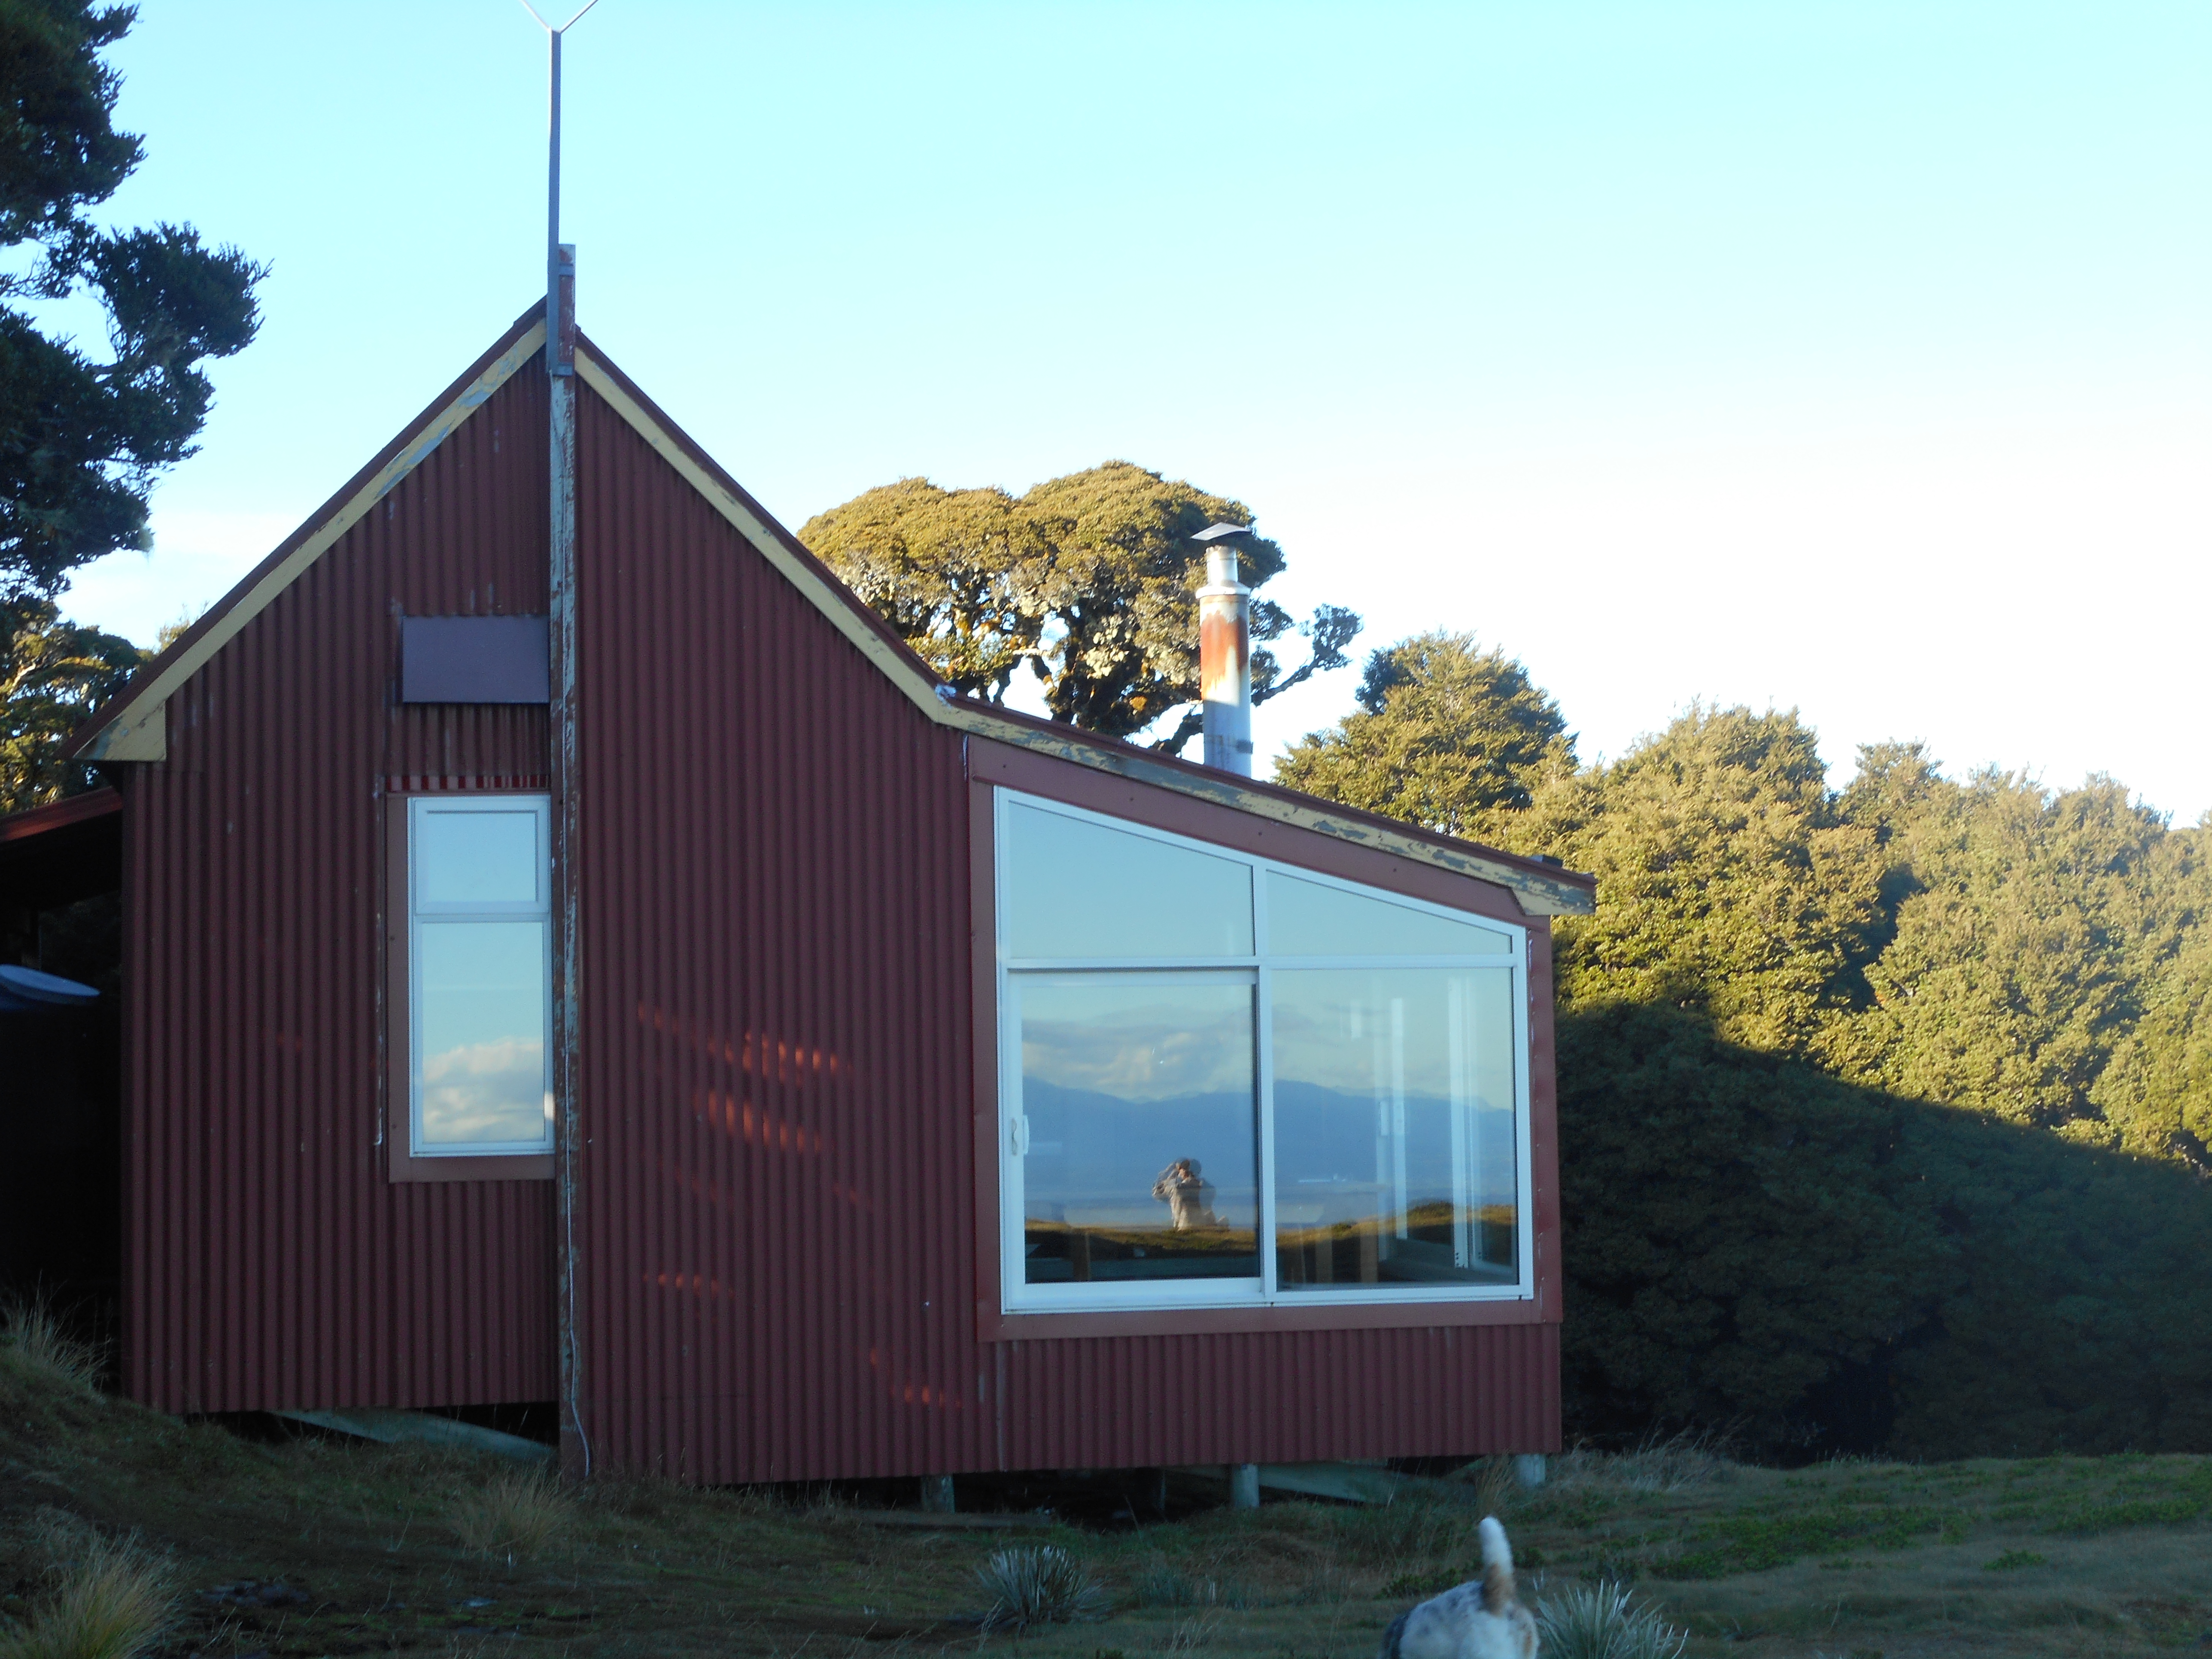
\includegraphics[width=8.5cm]{KirwansHut28May2017Photo1}
\end{flushleft}
\end{minipage}
\begin{minipage}{.5\linewidth}
\begin{flushright}
    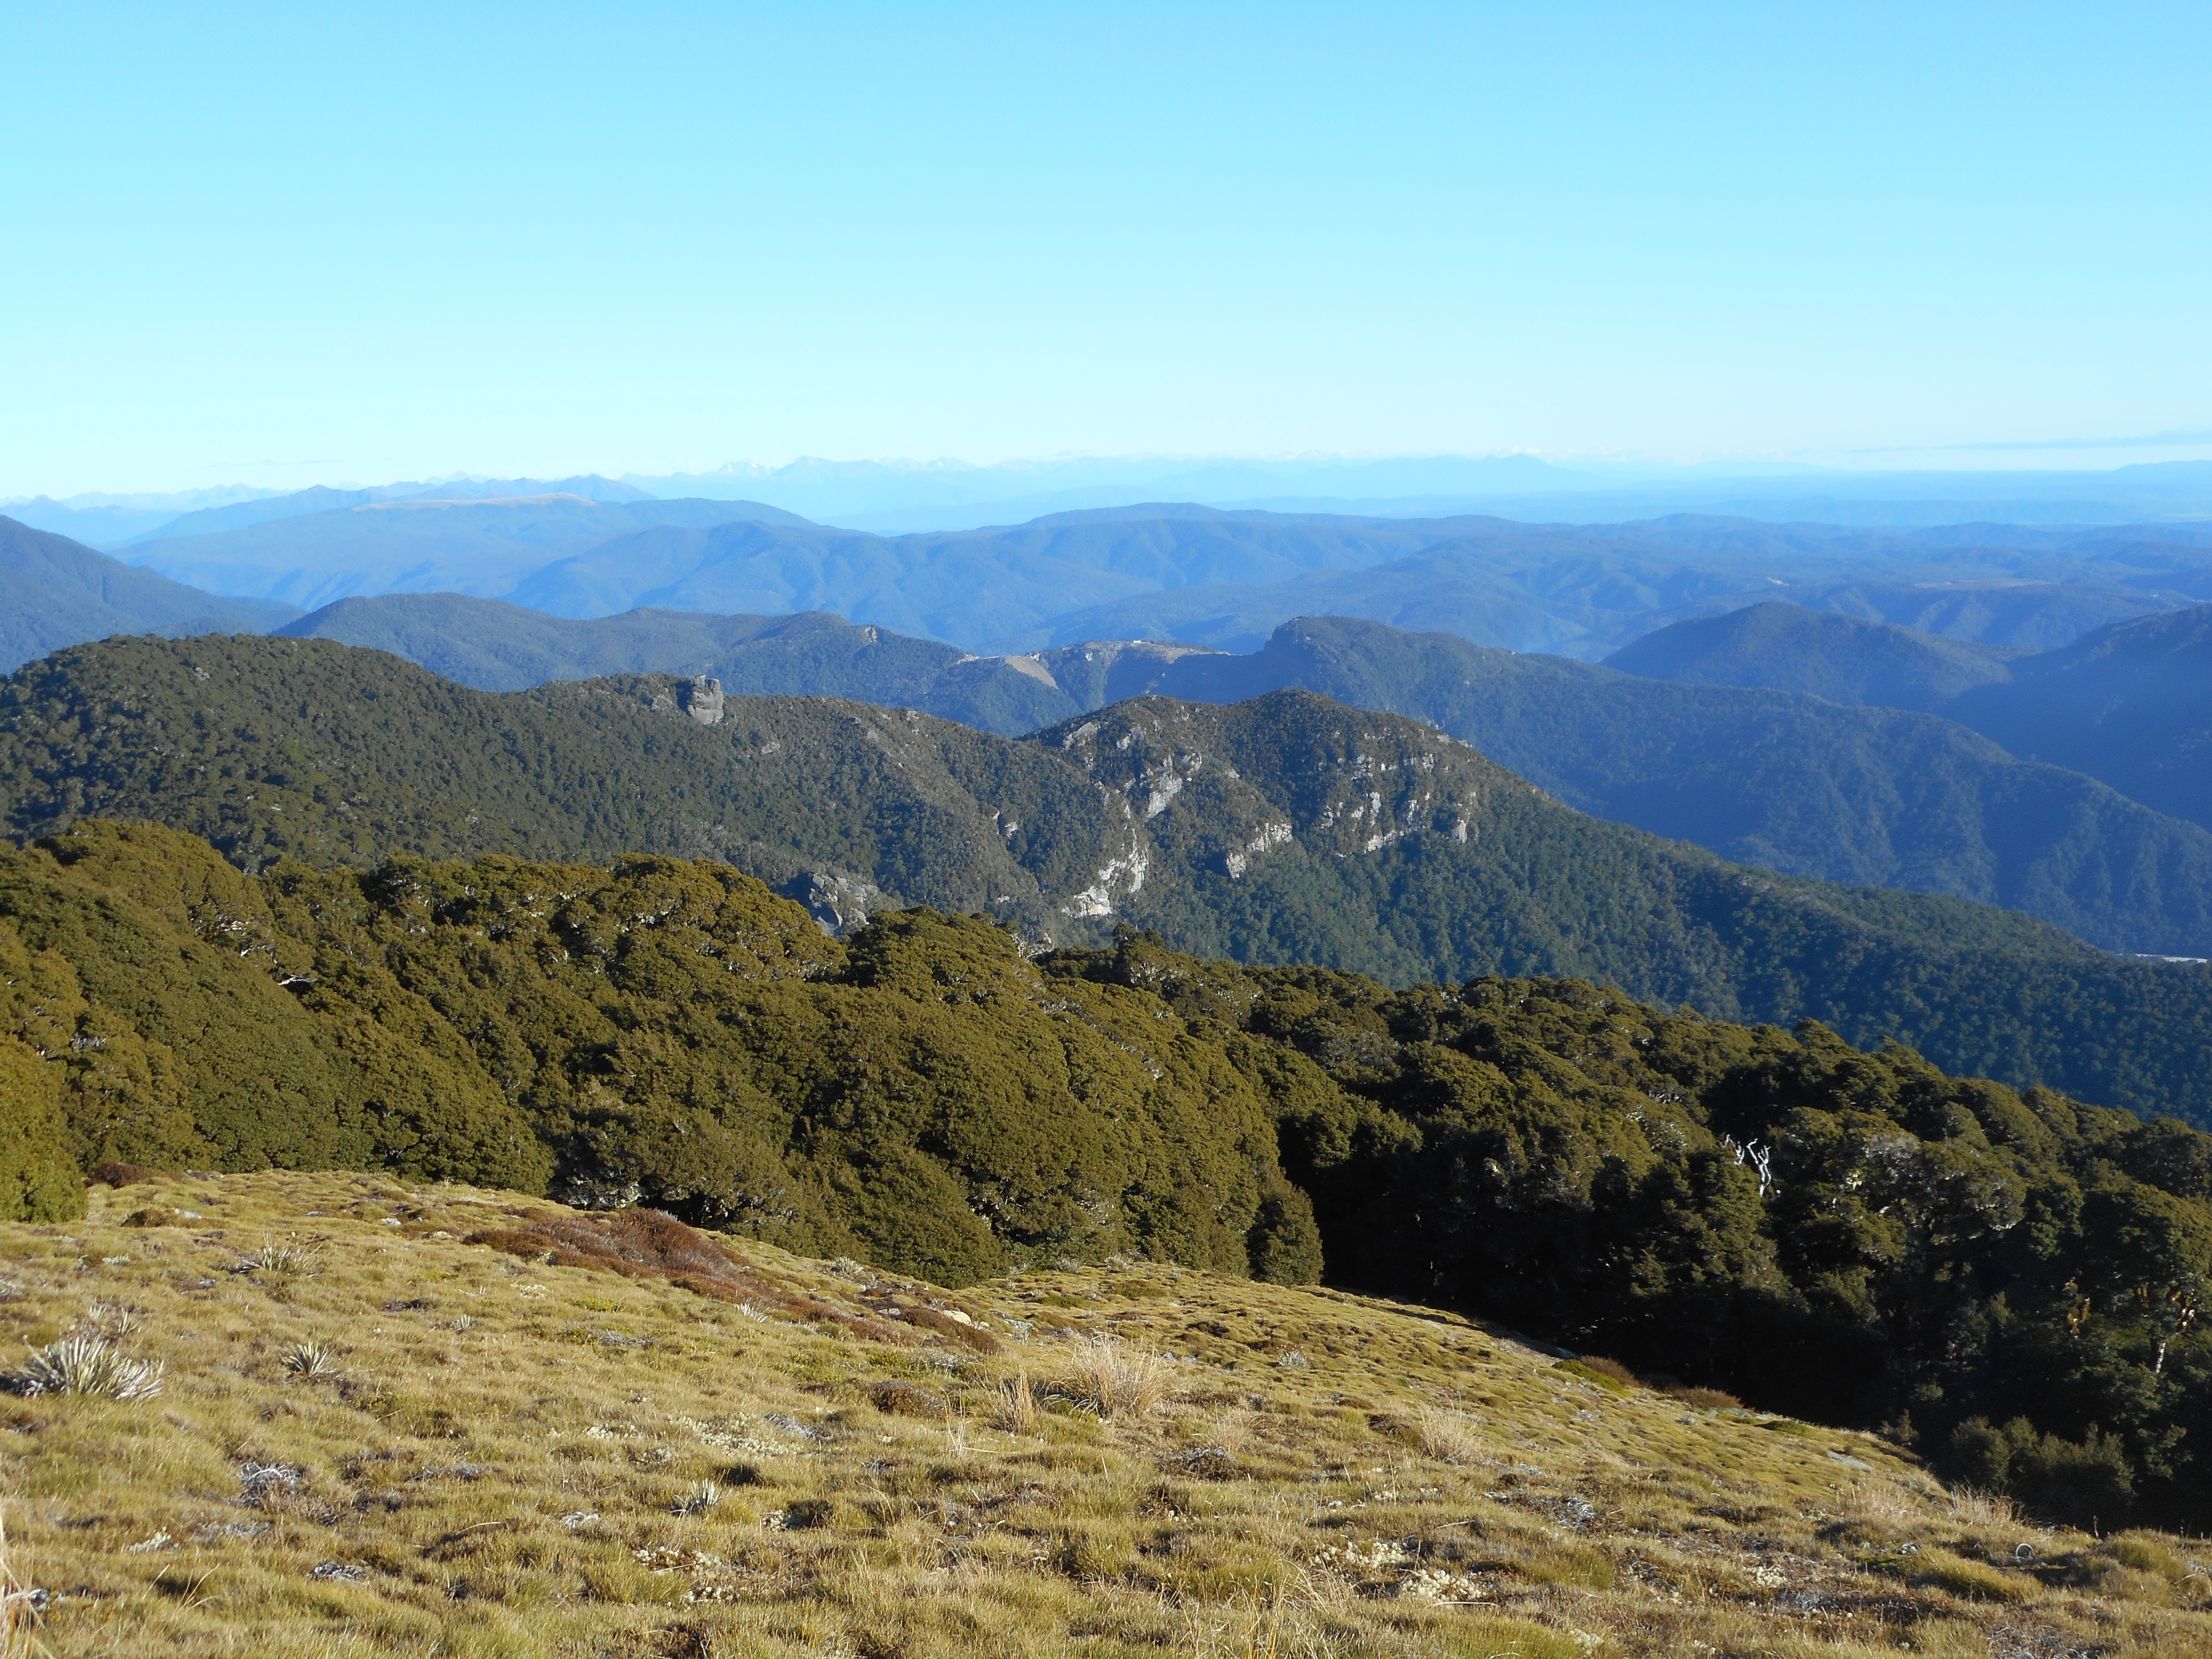
\includegraphics[width=8.5cm]{KirwansHut28May2017Photo2}
\end{flushright}
\end{minipage}

In the morning we left our packs at the turn off, and headed towards Montgomerie Hut for 5 or 10 minutes to look at the old mine site with the remnants of the aerial rope-way.  Upon resuming our walk out, we also took a detour to look at the  `Old Hut Site'.  We concluded that the hut was a miner's hut rather than an DoC or NZFS one.  With these diversions, which took about an hour, the total time (excluding lunch) for the return trip was about 4.25 hours.

\begin{minipage}{.55\linewidth}
\begin{flushleft}
   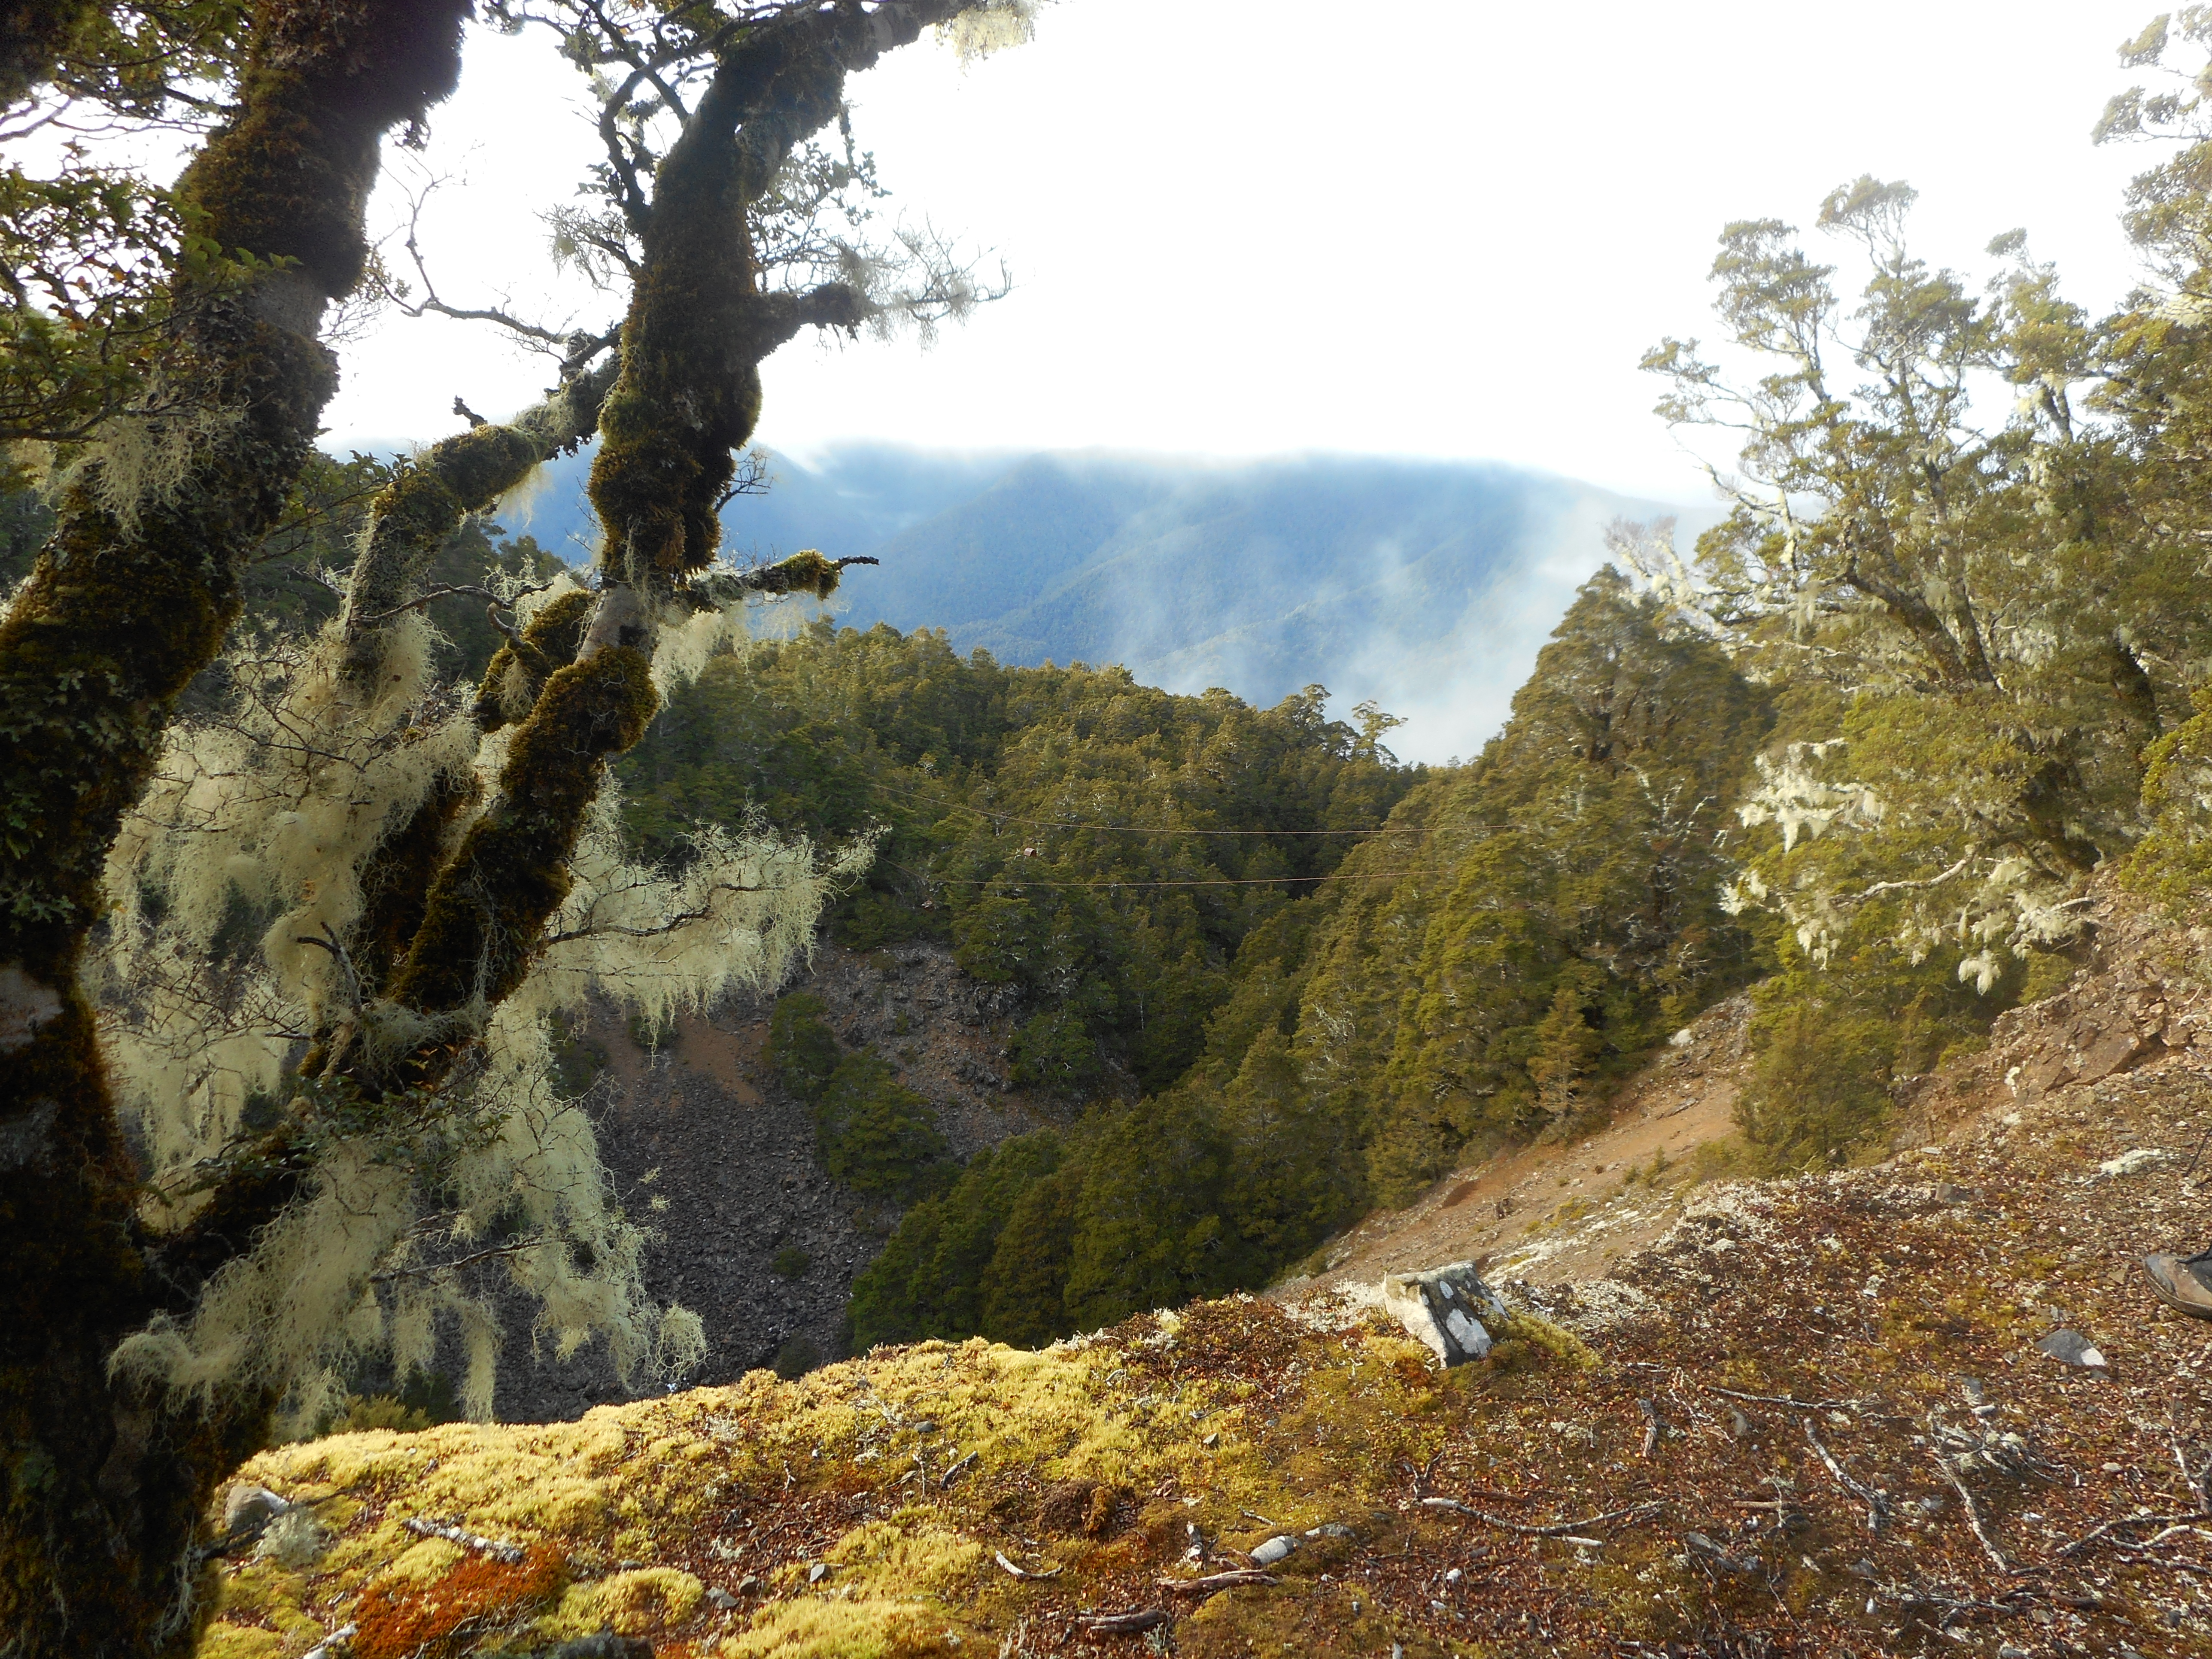
\includegraphics[width=9.5cm]{KirwansHut28May2017Photo3}
\end{flushleft}
\end{minipage}
\begin{minipage}{.45\linewidth}
\begin{flushright}
    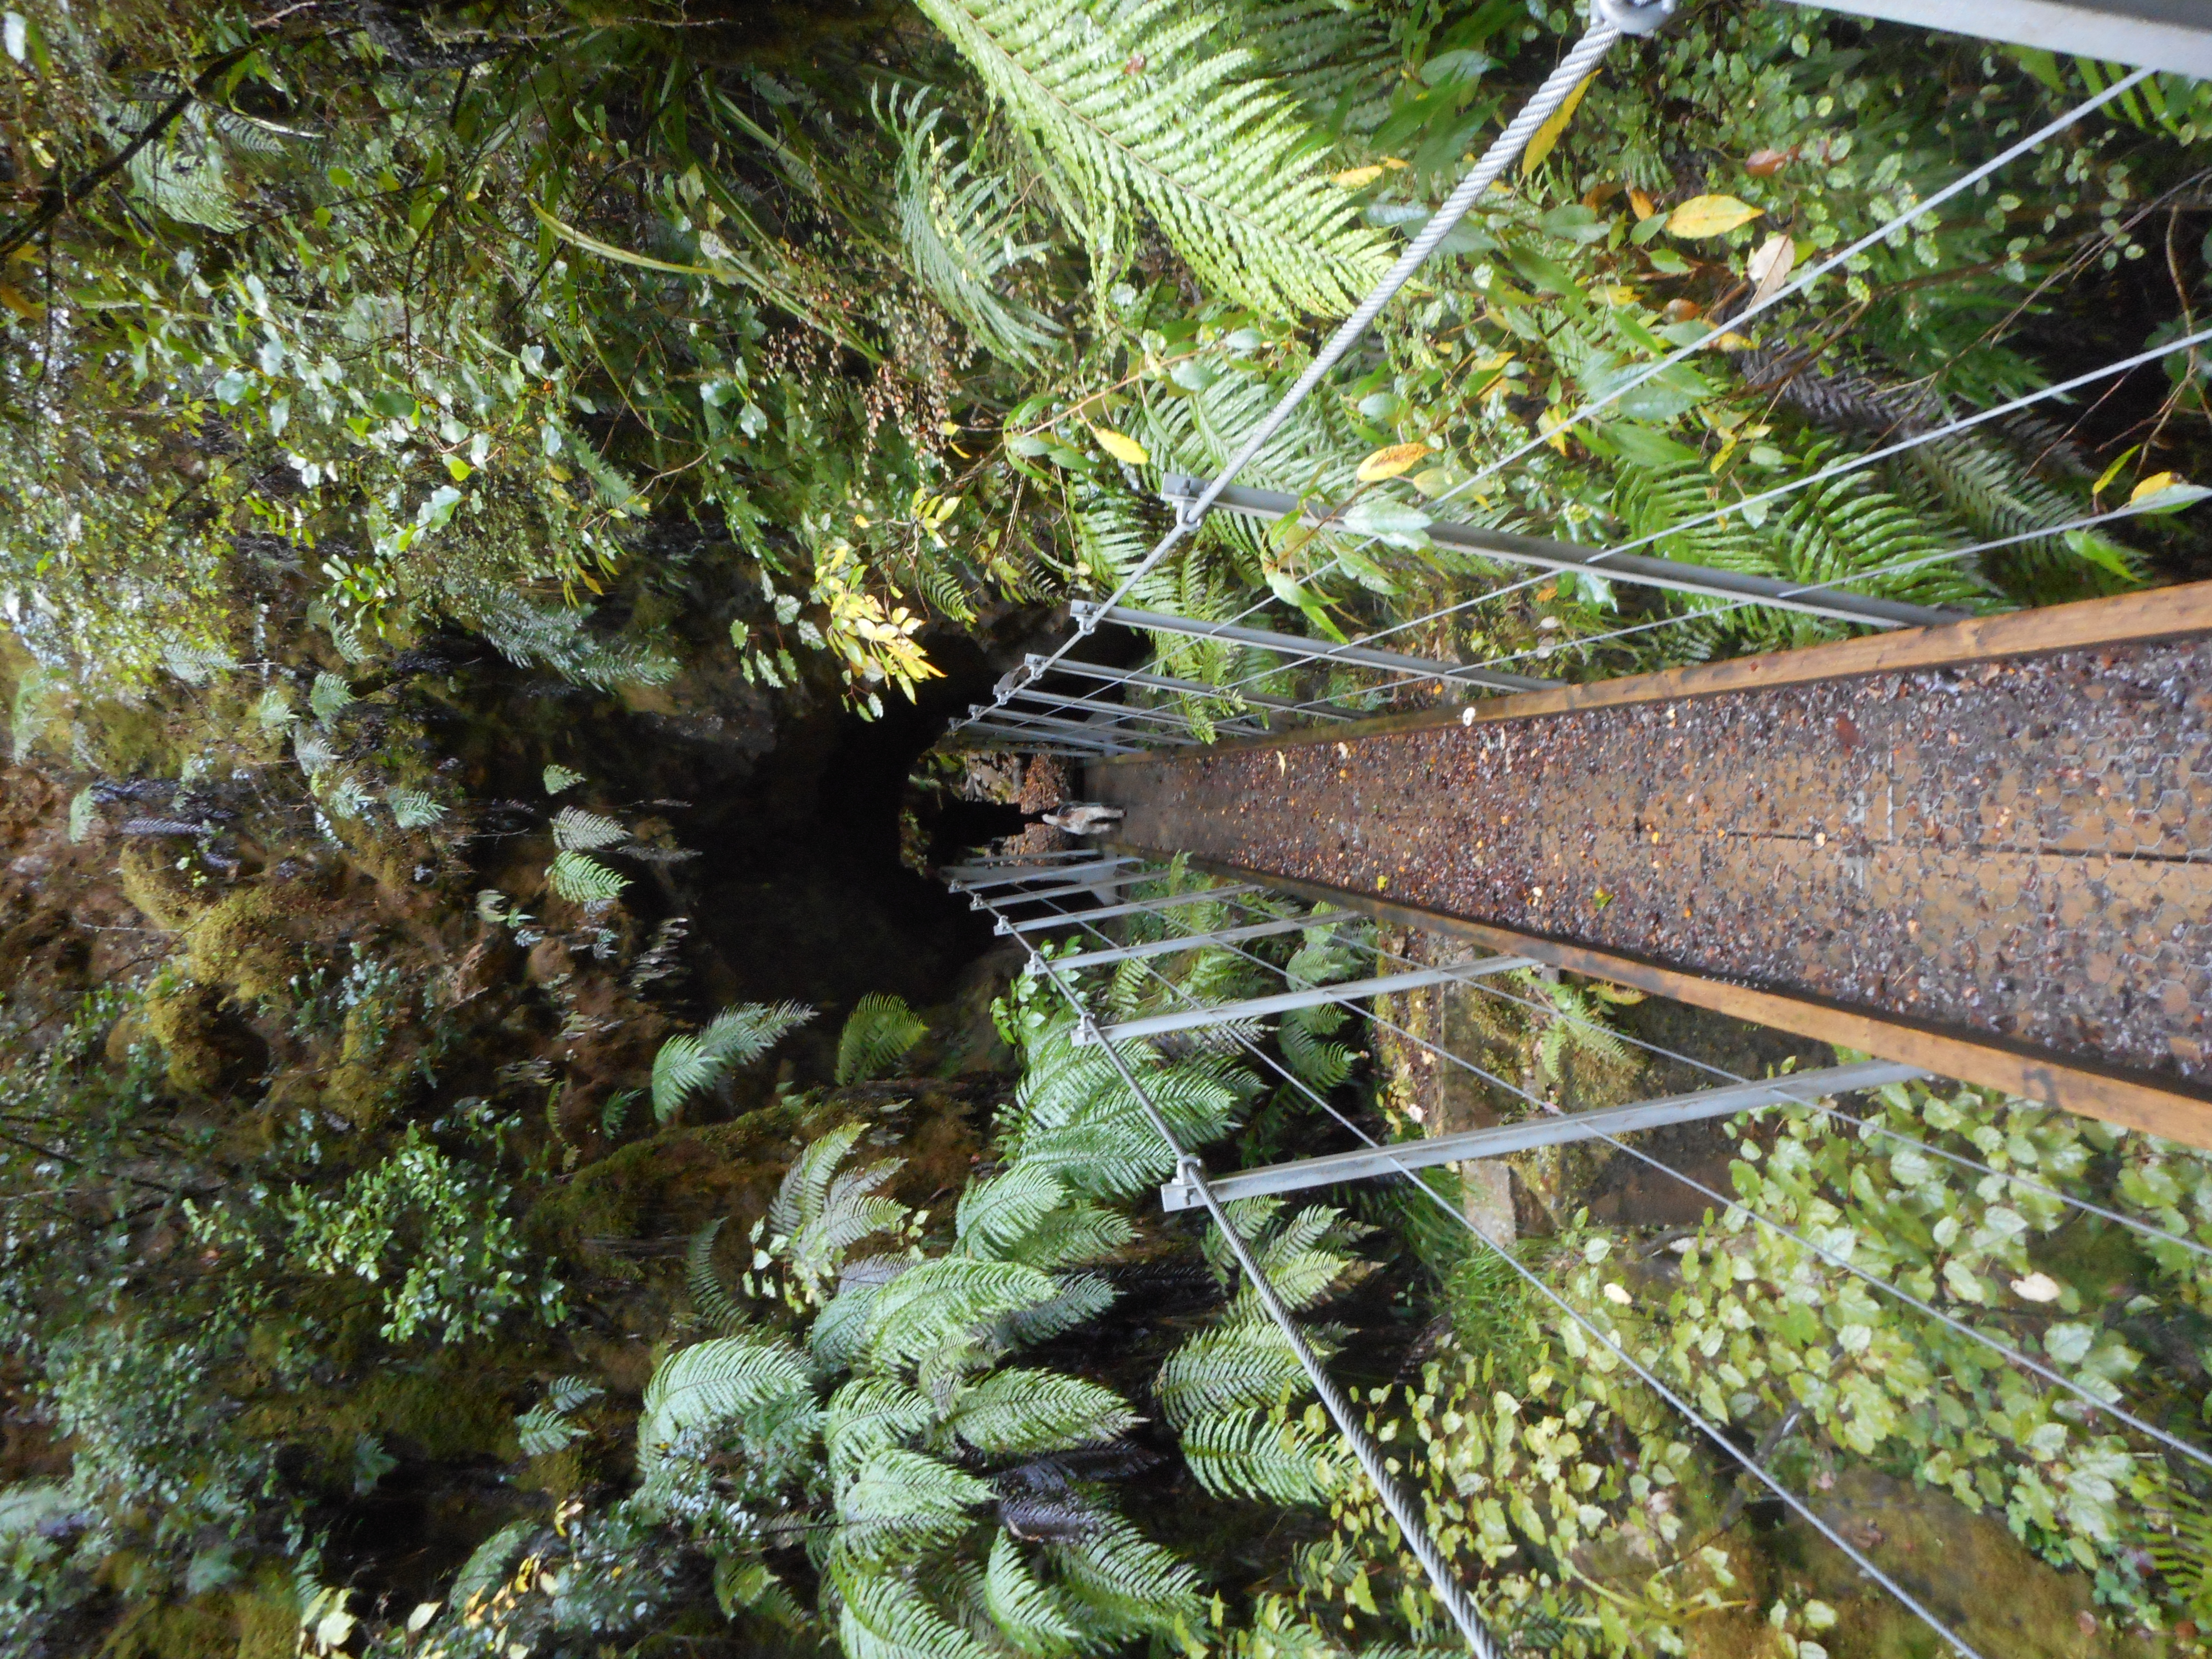
\includegraphics[width=9.5cm, angle=270]{KirwansHut28May2017Photo4}
\end{flushright}
\end{minipage}
\end{figure}

\begin{flushright}
Robyn, Peter and dog
\end{flushright}

\end{document}
